\documentclass[border=4pt]{standalone}
\usepackage{amsmath,amssymb}
\usepackage{tikz}
\usetikzlibrary{arrows.meta,shadows}
\begin{document}
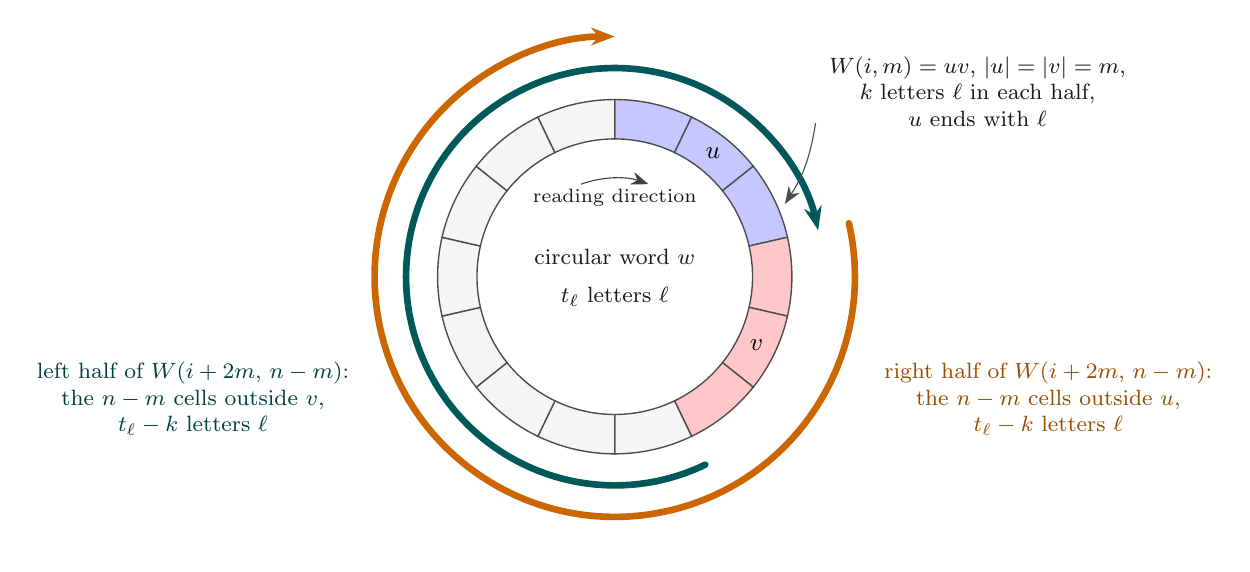
\begin{tikzpicture}[
  >={Stealth[length=2.2mm]},
  note/.style={font=\footnotesize,gray!20!black,align=center},
  hl/.style={line width=2.4pt,line cap=round}]
  \def\n{14}
  \def\ri{1.75}
  \def\ro{2.25}
  % cells of the circular word; cell s spans the angles th(s+1)..th(s), th(s) = 90 - 360 s / n
  \foreach \s in {0,...,13} {
    \pgfmathsetmacro{\a}{90-360*\s/\n}
    \pgfmathsetmacro{\b}{90-360*(\s+1)/\n}
    \ifnum\s<3 \def\col{blue!22}\else\ifnum\s<6 \def\col{red!22}\else\def\col{gray!8}\fi\fi
    \fill[\col,draw=gray!60!black,line width=0.5pt]
      (\a:\ri) arc[start angle=\a,end angle=\b,radius=\ri] -- (\b:\ro)
      arc[start angle=\b,end angle=\a,radius=\ro] -- cycle;
  }
  \node[font=\small] at ({90-360*1.5/\n}:2.0) {$u$};
  \node[font=\small] at ({90-360*4.5/\n}:2.0) {$v$};
  \node[note] at (0,0.25) {circular word $w$};
  \node[note] at (0,-0.25) {$t_\ell$ letters $\ell$};
  \draw[->,gray!50!black] (110:1.25) arc[start angle=110,end angle=70,radius=1.25];
  \node[note,font=\scriptsize] at (0,1.0) {reading direction};
  % the half-lengths
  \pgfmathsetmacro{\tA}{90}
  \pgfmathsetmacro{\tB}{90-360*3/\n}
  \pgfmathsetmacro{\tC}{90-360*6/\n}
  % left half of the mirror square: the complement of v
  \draw[hl,teal!70!black,-{Stealth[length=3mm]}] (\tC:2.65) arc[start angle=\tC,end angle={\tB-360},radius=2.65];
  % right half of the mirror square: the complement of u
  \draw[hl,orange!80!black,-{Stealth[length=3mm]}] (\tB:3.05) arc[start angle=\tB,end angle=-270,radius=3.05];
  \node[note,teal!50!black,anchor=east] at (-3.25,-1.55)
    {left half of $W(i+2m,\,n-m)$:\\ the $n-m$ cells outside $v$,\\ $t_\ell-k$ letters $\ell$};
  \node[note,orange!60!black,anchor=west] at (3.3,-1.55)
    {right half of $W(i+2m,\,n-m)$:\\ the $n-m$ cells outside $u$,\\ $t_\ell-k$ letters $\ell$};
  \node[note,anchor=west] at (2.6,2.35)
    {$W(i,m)=uv$, $|u|=|v|=m$,\\ $k$ letters $\ell$ in each half,\\ $u$ ends with $\ell$};
  \draw[->,gray!60!black] (2.55,1.95) to[bend left=12] ({90-360*2.6/\n}:2.35);
\end{tikzpicture}
\end{document}
